\newcommand{\xmmm}{.7}
\newcommand{\smT}{.45}
\newcommand{\lgT}{.85}

\begin{center}
    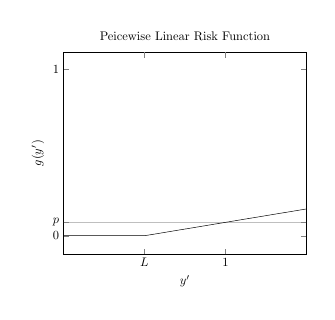
\begin{tikzpicture}[scale=\smT]
      \begin{axis}[ 
	  xlabel=$y'$,
	  ylabel=$g(y')$,
	  title = Peicewise Linear Risk Function,
	  unbounded coords = jump,
	  xtick= {0},
	  ytick= {0, 1},
	  extra y ticks={.08},
	  extra y tick style={grid=major},
	  extra y tick labels={$p$},
	  extra x ticks={.9,1,1.4},
	  extra x tick labels={$L$, 1, $U^c$},
          xmin=.8,
          xmax=1.1,
          ymax=1.1,
          scatter/classes={
 	    a={mark=o,line width=3pt,scale=.75},%
 	    b={mark=o,line width=1pt,scale=1.25}%
	}]
	\addplot[black] coordinates { 
	  (0,0)		
	  (.9,0)	
	  (1.3975,.3995)		
	};	
        \addplot[black,mark=x,mark size=1pt] coordinates { (1.4,1) (2.5, 1)};
        \addplot[black,mark=o,mark size=1.4pt] coordinates{(1.4,.4)};
      \end{axis}
    \end{tikzpicture}
\begin{tikzpicture}[scale=\lgT]
\begin{axis}[title=L vs Risk (\textbf{linear}), xlabel=L, ylabel=r,legend pos=outer north east,ymax=.04,xmin=\xmmm,xmax=1,
	  extra x ticks={.8,.9,.98},
	  extra x tick style={grid=major},
	  extra x tick labels={}]


  \addplot+[opacity=.65,color=black,only marks, mark size=.35] table[x=L,y=opf] {\mypathjccdata/linear.dat};
  \addlegendentryexpanded{OPF}

  \addplot+[opacity=.65,color=red,only marks, mark size=.35] table[x=L,y=cc] {\mypathjccdata/linear.dat};
  \addlegendentryexpanded{CC .01}


  \addplot+[opacity=.65,color=red!60,only marks, mark size=.35] table[x=L,y=cc] {\mypathjccdata/linear-CC.dat};
  \addlegendentryexpanded{CC .05}


  \addplot+[opacity=.65,color=blue!40,only marks, mark size=.35] table[x=L,y=jcc] {\mypathjccdata/linear-L2.dat};
  \addlegendentryexpanded{JCC .8}

  \addplot+[opacity=.65,only marks,color=blue!60, mark size=.35] table[x=L,y=jcc] {\mypathjccdata/linear-L.dat};
  \addlegendentryexpanded{JCC .9}

  \addplot+[opacity=.65,only marks,color=blue!80, mark size=.35] table[x=L,y=jcc] {\mypathjccdata/linear.dat};
  \addlegendentryexpanded{JCC .98}

\end{axis}
\end{tikzpicture}

    \begin{tikzpicture}[scale=\smT]
      \begin{axis}[ 
	  xlabel=$y'$,
	  ylabel=$g(y')$,
	  title = Square,
	  unbounded coords = jump,
	  xtick= {0},
	  ytick= {0, 1},
	  extra y ticks={.08},
	  extra y tick style={grid=major},
	  extra y tick labels={$p$},
	  extra x ticks={.9,1,1.4},
	  extra x tick labels={$L$, 1, $U^c$},
          xmin=.8,
          xmax=1.1,
          ymax=1.1,
          scatter/classes={
 	    a={mark=o,line width=3pt,scale=.75},%
 	    b={mark=o,line width=1pt,scale=1.25}%
	}]
	\addplot[black] coordinates { 
	  (0,0)		
	  (.9,0)	
	};	
	\addplot[black, domain=.9:1.3975,samples=100] { .08*((x-.9)/(.1))^2	};	
        \addplot[black,mark=x,mark size=1pt] coordinates { (1.4,1) (2.5, 1)};
        \addplot[black,mark=o,mark size=1.4pt] coordinates{(1.4,.4)};
      \end{axis}
    \end{tikzpicture}
\begin{tikzpicture}[scale=\lgT]
\begin{axis}[title=L vs Risk (\textbf{square}), xlabel=L, ylabel=r,legend pos=outer north east,ymax=.04,xmin=\xmmm,xmax=1,
	  extra x ticks={.8,.9,.98},
	  extra x tick style={grid=major},
	  extra x tick labels={}]


  \addplot+[opacity=.65,only marks, mark size=.35, color=black] table[x=L,y=opf] {\mypathjccdata/square.dat};
  \addlegendentryexpanded{OPF}

  \addplot+[opacity=.65,only marks, mark size=.35, color=red] table[x=L,y=cc] {\mypathjccdata/square.dat};
  \addlegendentryexpanded{CC .01}

  \addplot+[opacity=.65,color=red!60,only marks, mark size=.35] table[x=L,y=cc] {\mypathjccdata/square-CC.dat};
  \addlegendentryexpanded{CC .05}

  \addplot+[opacity=.65,color=blue!40,only marks, mark size=.35] table[x=L,y=jcc] {\mypathjccdata/square-L2.dat};
  \addlegendentryexpanded{JCC .8}

  \addplot+[opacity=.65,only marks,color=blue!60, mark size=.35] table[x=L,y=jcc] {\mypathjccdata/square-L.dat};
  \addlegendentryexpanded{JCC .9}

  \addplot+[opacity=.65,only marks, color=blue!80, mark size=.35] table[x=L,y=jcc] {\mypathjccdata/square.dat};
  \addlegendentryexpanded{JCC .98}

\end{axis}
\end{tikzpicture}

    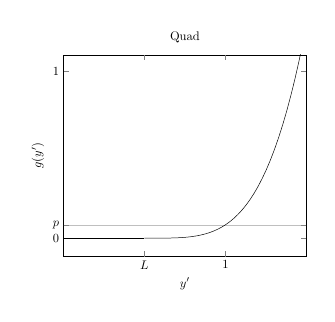
\begin{tikzpicture}[scale=\smT]
      \begin{axis}[ 
	  xlabel=$y'$,
	  ylabel=$g(y')$,
	  title = Quad,
	  unbounded coords = jump,
	  xtick= {0},
	  ytick= {0, 1},
	  extra y ticks={.08},
	  extra y tick style={grid=major},
	  extra y tick labels={$p$},
	  extra x ticks={.9,1,1.4},
	  extra x tick labels={$L$, 1, $U^c$},
          xmin=.8,
          xmax=1.1,
          ymax=1.1,
          scatter/classes={
 	    a={mark=o,line width=3pt,scale=.75},%
 	    b={mark=o,line width=1pt,scale=1.25}%
	}]
	\addplot[black] coordinates { 
	  (0,0)		
	  (.9,0)	
	};	
	\addplot[black, domain=.9:1.3975,samples=100] { .08*((x-.9)/(.1))^4	};	
        \addplot[black,mark=x,mark size=1pt] coordinates { (1.4,1) (2.5, 1)};
        \addplot[black,mark=o,mark size=1.4pt] coordinates{(1.4,.4)};
      \end{axis}
    \end{tikzpicture}
\begin{tikzpicture}[scale=\lgT]
\begin{axis}[title=L vs Risk (\textbf{quad}), xlabel=L, ylabel=r,legend pos=outer north east,ymax=.04,xmin=\xmmm,xmax=1,
	  extra x ticks={.8,.9,.98},
	  extra x tick style={grid=major},
	  extra x tick labels={}]


  \addplot+[opacity=.65,only marks, mark size=.35,color=black] table[x=L,y=opf] {\mypathjccdata/quad.dat};
  \addlegendentryexpanded{OPF}

  \addplot+[opacity=.65,only marks, mark size=.35,color=red] table[x=L,y=cc] {\mypathjccdata/quad.dat};
  \addlegendentryexpanded{CC .01}
  \addplot+[opacity=.65,color=red!60,only marks, mark size=.35] table[x=L,y=cc] {\mypathjccdata/quad-CC.dat};
  \addlegendentryexpanded{CC .05}

  \addplot+[opacity=.65,color=blue!40,only marks, mark size=.35] table[x=L,y=jcc] {\mypathjccdata/quad-L2.dat};
  \addlegendentryexpanded{JCC .8}

  \addplot+[opacity=.65,only marks,color=blue!60, mark size=.35] table[x=L,y=jcc] {\mypathjccdata/quad-L.dat};
  \addlegendentryexpanded{JCC .9}

  \addplot+[opacity=.65,only marks, mark size=.35,color=blue!80] table[x=L,y=jcc] {\mypathjccdata/quad.dat};
  \addlegendentryexpanded{JCC .98}

\end{axis}
\end{tikzpicture}
\end{center}
